\chapter{Artificial Neural Nets - Supervised Learning: Classification }
% Authors: Colin Andrus , Aakriti Gupta, Daniel Rivera, 2/11/18.

\section{Example of Not Linearly Separable Curves}


We have three curves defined by functions:
\[X_c(t) = t
\begin{pmatrix}
    sin( \frac{2 \pi}{C}(2t + c -1)) \\
    cos( \frac{2 \pi}{C}(2t + c -1))
\end{pmatrix}
 \]
\[ 0 \leq t \leq 1 \quad c = 1,..., C\]

\begin{figure}[h]
    \centering
    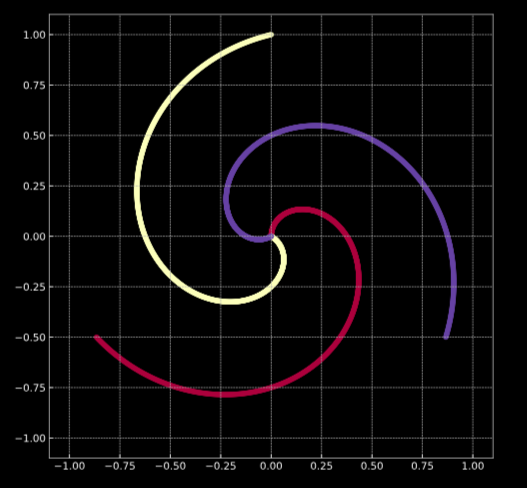
\includegraphics[width=200pt]{labs/02/images/spiral1.png}
    \caption{3 Not Linearly Separable Parametric Curves}
    \label{fig:my_label}
\end{figure}


We cannot linearly separate the data points in these curves as shown in the figure below.  These points are defined by the same function with added noise.

\[X_c(t) = t
\begin{pmatrix}
    sin( \frac{2 \pi}{C}(2t + c -1) + \mathcal{N} (0, \sigma ^2 )) \\
    cos( \frac{2 \pi}{C}(2t + c -1) + \mathcal{N} (0, \sigma ^2 ) )
\end{pmatrix}
 \]
\[ 0 \leq t \leq 1 \quad c = 1,..., C\]